\documentclass{standalone}
\usepackage{tikz}
\usetikzlibrary{patterns, positioning}
\usepackage[sfdefault]{ClearSans} %% option 'sfdefault' activates Clear Sans as the default text font
\usepackage[T1]{fontenc}

\begin{document}
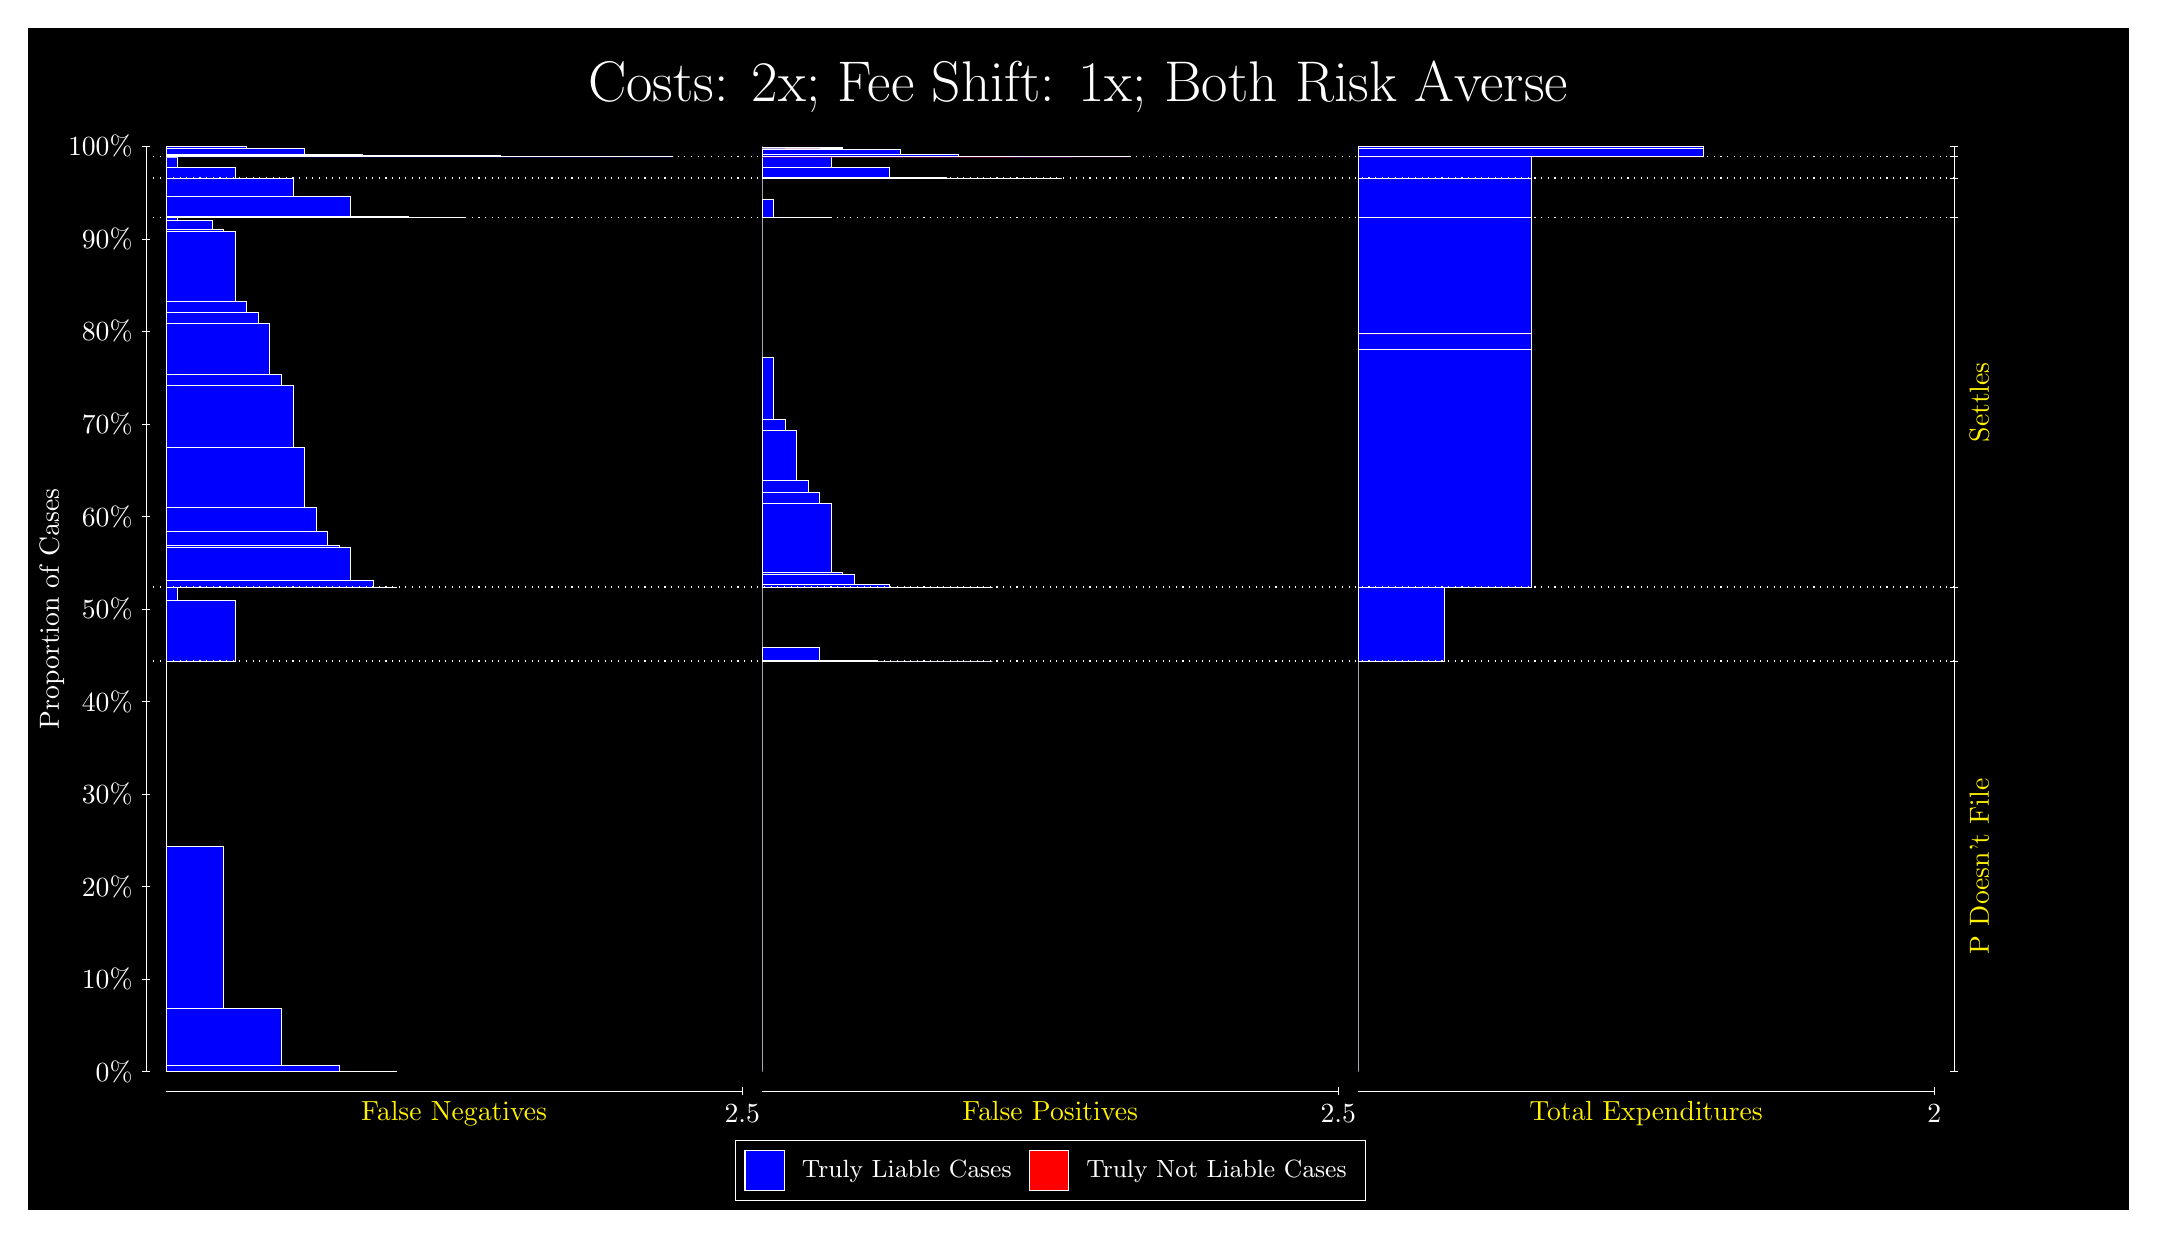
\begin{tikzpicture}
\draw[fill=black] (0,0) rectangle (26.667,15);
\draw[text=white] (0,13.5) rectangle (26.667,15) node[midway] {\huge Costs: 2x; Fee Shift: 1x; Both Risk Averse};
\draw[white, very thin] (1.5,1.75) -- (1.5,13.5);
\node[rotate=90, text=white, anchor=center] at (0.3, 7.625) {Proportion of Cases};
\draw[white, very thin] (1.45,1.75) -- (1.55,1.75);
\node[text=white, anchor=east] at (1.45, 1.75) {0\%};
\draw[white, very thin] (1.45,2.925) -- (1.55,2.925);
\node[text=white, anchor=east] at (1.45, 2.925) {10\%};
\draw[white, very thin] (1.45,4.1) -- (1.55,4.1);
\node[text=white, anchor=east] at (1.45, 4.1) {20\%};
\draw[white, very thin] (1.45,5.275) -- (1.55,5.275);
\node[text=white, anchor=east] at (1.45, 5.275) {30\%};
\draw[white, very thin] (1.45,6.45) -- (1.55,6.45);
\node[text=white, anchor=east] at (1.45, 6.45) {40\%};
\draw[white, very thin] (1.45,7.625) -- (1.55,7.625);
\node[text=white, anchor=east] at (1.45, 7.625) {50\%};
\draw[white, very thin] (1.45,8.8) -- (1.55,8.8);
\node[text=white, anchor=east] at (1.45, 8.8) {60\%};
\draw[white, very thin] (1.45,9.975) -- (1.55,9.975);
\node[text=white, anchor=east] at (1.45, 9.975) {70\%};
\draw[white, very thin] (1.45,11.15) -- (1.55,11.15);
\node[text=white, anchor=east] at (1.45, 11.15) {80\%};
\draw[white, very thin] (1.45,12.325) -- (1.55,12.325);
\node[text=white, anchor=east] at (1.45, 12.325) {90\%};
\draw[white, very thin] (1.45,13.5) -- (1.55,13.5);
\node[text=white, anchor=east] at (1.45, 13.5) {100\%};

\draw[white, very thin] (24.457,1.75) -- (24.457,13.5);
\draw[white, very thin] (24.407,1.75) -- (24.507,1.75);
\node[anchor=west] at (24.407, 1.75) {};
\draw[white, very thin] (24.407,6.9636) -- (24.507,6.9636);
\node[anchor=west] at (24.407, 6.9636) {};
\draw[white, very thin] (24.407,7.9029) -- (24.507,7.9029);
\node[anchor=west] at (24.407, 7.9029) {};
\draw[white, very thin] (24.407,12.597) -- (24.507,12.597);
\node[anchor=west] at (24.407, 12.597) {};
\draw[white, very thin] (24.407,13.098) -- (24.507,13.098);
\node[anchor=west] at (24.407, 13.098) {};
\draw[white, very thin] (24.407,13.37) -- (24.507,13.37);
\node[anchor=west] at (24.407, 13.37) {};
\draw[white, very thin] (24.407,13.5) -- (24.507,13.5);
\node[anchor=west] at (24.407, 13.5) {};

\draw[white, very thin, fill=blue] (1.75,1.75) rectangle (4.6775,1.7508);
\draw[white, very thin, fill=blue] (1.75,1.7508) rectangle (3.9457,1.835);
\draw[white, very thin, fill=blue] (1.75,1.835) rectangle (3.2138,2.5588);
\draw[white, very thin, fill=blue] (1.75,2.5588) rectangle (2.4819,4.6165);
\draw[white, very thin, fill=red] (1.75,4.6165) rectangle (1.75,4.6165);
\draw[white, very thin, fill=blue] (1.75,4.6165) rectangle (1.75,6.9636);
\draw[white, very thin, fill=blue] (1.75,6.9636) rectangle (2.6283,7.7329);
\draw[white, very thin, fill=blue] (1.75,7.7329) rectangle (1.8964,7.8983);
\draw[white, very thin, fill=red] (1.75,7.8983) rectangle (1.75,7.8983);
\draw[white, very thin, fill=blue] (1.75,7.8983) rectangle (1.75,7.9029);
\draw[white, very thin, fill=blue] (1.75,7.9029) rectangle (4.6775,7.903);
\draw[white, very thin, fill=blue] (1.75,7.903) rectangle (4.3848,7.9842);
\draw[white, very thin, fill=blue] (1.75,7.9842) rectangle (4.092,8.4039);
\draw[white, very thin, fill=blue] (1.75,8.4039) rectangle (3.9457,8.4383);
\draw[white, very thin, fill=blue] (1.75,8.4383) rectangle (3.7993,8.6117);
\draw[white, very thin, fill=blue] (1.75,8.6117) rectangle (3.6529,8.9181);
\draw[white, very thin, fill=blue] (1.75,8.9181) rectangle (3.5065,9.683);
\draw[white, very thin, fill=blue] (1.75,9.683) rectangle (3.3602,10.467);
\draw[white, very thin, fill=blue] (1.75,10.467) rectangle (3.2138,10.602);
\draw[white, very thin, fill=blue] (1.75,10.602) rectangle (3.0674,11.247);
\draw[white, very thin, fill=blue] (1.75,11.247) rectangle (2.921,11.394);
\draw[white, very thin, fill=blue] (1.75,11.394) rectangle (2.7746,11.529);
\draw[white, very thin, fill=blue] (1.75,11.529) rectangle (2.6283,12.415);
\draw[white, very thin, fill=blue] (1.75,12.415) rectangle (2.4819,12.441);
\draw[white, very thin, fill=blue] (1.75,12.441) rectangle (2.3355,12.558);
\draw[white, very thin, fill=blue] (1.75,12.558) rectangle (2.1891,12.563);
\draw[white, very thin, fill=blue] (1.75,12.563) rectangle (2.0428,12.564);
\draw[white, very thin, fill=blue] (1.75,12.564) rectangle (1.8964,12.597);
\draw[white, very thin, fill=red] (1.75,12.597) rectangle (1.75,12.597);
\draw[white, very thin, fill=blue] (1.75,12.597) rectangle (1.75,12.597);
\draw[white, very thin, fill=blue] (1.75,12.597) rectangle (5.5558,12.597);
\draw[white, very thin, fill=blue] (1.75,12.597) rectangle (4.8239,12.606);
\draw[white, very thin, fill=blue] (1.75,12.606) rectangle (4.092,12.869);
\draw[white, very thin, fill=blue] (1.75,12.869) rectangle (3.3602,13.096);
\draw[white, very thin, fill=blue] (1.75,13.096) rectangle (2.6283,13.098);
\draw[white, very thin, fill=red] (1.75,13.098) rectangle (1.75,13.098);
\draw[white, very thin, fill=blue] (1.75,13.098) rectangle (2.6283,13.237);
\draw[white, very thin, fill=blue] (1.75,13.237) rectangle (1.8964,13.367);
\draw[white, very thin, fill=red] (1.75,13.367) rectangle (1.75,13.367);
\draw[white, very thin, fill=blue] (1.75,13.367) rectangle (1.75,13.37);
\draw[white, very thin, fill=blue] (1.75,13.37) rectangle (8.1906,13.37);
\draw[white, very thin, fill=blue] (1.75,13.37) rectangle (7.4587,13.37);
\draw[white, very thin, fill=blue] (1.75,13.37) rectangle (6.7268,13.373);
\draw[white, very thin, fill=blue] (1.75,13.373) rectangle (5.9949,13.387);
\draw[white, very thin, fill=blue] (1.75,13.387) rectangle (5.7022,13.387);
\draw[white, very thin, fill=blue] (1.75,13.387) rectangle (5.2631,13.388);
\draw[white, very thin, fill=blue] (1.75,13.388) rectangle (4.9703,13.389);
\draw[white, very thin, fill=blue] (1.75,13.389) rectangle (4.5312,13.389);
\draw[white, very thin, fill=blue] (1.75,13.389) rectangle (4.2384,13.405);
\draw[white, very thin, fill=blue] (1.75,13.405) rectangle (3.7993,13.405);
\draw[white, very thin, fill=blue] (1.75,13.405) rectangle (3.5065,13.469);
\draw[white, very thin, fill=blue] (1.75,13.469) rectangle (2.7746,13.498);
\draw[white, very thin, fill=blue] (1.75,13.498) rectangle (2.0428,13.5);
\draw[white, very thin, fill=red] (1.75,13.5) rectangle (1.75,13.5);
\draw[white, very thin, fill=blue] (1.75,13.5) rectangle (1.75,13.5);
\draw[white, very thin, fill=red] (9.3189,1.75) rectangle (9.3189,1.75);
\draw[white, very thin, fill=blue] (9.3189,1.75) rectangle (9.3189,6.9636);
\draw[white, very thin, fill=red] (9.3189,6.9636) rectangle (12.246,6.9636);
\draw[white, very thin, fill=blue] (9.3189,6.9636) rectangle (12.246,6.9636);
\draw[white, very thin, fill=blue] (9.3189,6.9636) rectangle (11.515,6.9636);
\draw[white, very thin, fill=blue] (9.3189,6.9636) rectangle (10.783,6.9681);
\draw[white, very thin, fill=blue] (9.3189,6.9681) rectangle (10.051,7.1336);
\draw[white, very thin, fill=blue] (9.3189,7.1336) rectangle (9.3189,7.9029);
\draw[white, very thin, fill=red] (9.3189,7.9029) rectangle (12.246,7.9029);
\draw[white, very thin, fill=blue] (9.3189,7.9029) rectangle (12.246,7.9029);
\draw[white, very thin, fill=red] (9.3189,7.9029) rectangle (11.954,7.9029);
\draw[white, very thin, fill=blue] (9.3189,7.9029) rectangle (11.954,7.9029);
\draw[white, very thin, fill=red] (9.3189,7.9029) rectangle (11.661,7.9029);
\draw[white, very thin, fill=blue] (9.3189,7.9029) rectangle (11.661,7.9029);
\draw[white, very thin, fill=blue] (9.3189,7.9029) rectangle (11.515,7.9029);
\draw[white, very thin, fill=red] (9.3189,7.9029) rectangle (11.368,7.9029);
\draw[white, very thin, fill=blue] (9.3189,7.9029) rectangle (11.368,7.9029);
\draw[white, very thin, fill=blue] (9.3189,7.9029) rectangle (11.222,7.9031);
\draw[white, very thin, fill=red] (9.3189,7.9031) rectangle (11.075,7.9031);
\draw[white, very thin, fill=blue] (9.3189,7.9031) rectangle (11.075,7.9032);
\draw[white, very thin, fill=blue] (9.3189,7.9032) rectangle (10.929,7.9364);
\draw[white, very thin, fill=blue] (9.3189,7.9364) rectangle (10.783,7.9371);
\draw[white, very thin, fill=blue] (9.3189,7.9371) rectangle (10.636,7.9419);
\draw[white, very thin, fill=blue] (9.3189,7.9419) rectangle (10.49,8.0594);
\draw[white, very thin, fill=blue] (9.3189,8.0594) rectangle (10.344,8.0848);
\draw[white, very thin, fill=blue] (9.3189,8.0848) rectangle (10.197,8.9711);
\draw[white, very thin, fill=blue] (9.3189,8.9711) rectangle (10.051,9.1063);
\draw[white, very thin, fill=blue] (9.3189,9.1063) rectangle (9.9044,9.2531);
\draw[white, very thin, fill=blue] (9.3189,9.2531) rectangle (9.758,9.8984);
\draw[white, very thin, fill=blue] (9.3189,9.8984) rectangle (9.6116,10.033);
\draw[white, very thin, fill=blue] (9.3189,10.033) rectangle (9.4652,10.817);
\draw[white, very thin, fill=blue] (9.3189,10.817) rectangle (9.3189,12.597);
\draw[white, very thin, fill=red] (9.3189,12.597) rectangle (10.197,12.597);
\draw[white, very thin, fill=blue] (9.3189,12.597) rectangle (10.197,12.6);
\draw[white, very thin, fill=blue] (9.3189,12.6) rectangle (9.4652,12.827);
\draw[white, very thin, fill=blue] (9.3189,12.827) rectangle (9.3189,13.098);
\draw[white, very thin, fill=red] (9.3189,13.098) rectangle (13.125,13.098);
\draw[white, very thin, fill=blue] (9.3189,13.098) rectangle (13.125,13.098);
\draw[white, very thin, fill=blue] (9.3189,13.098) rectangle (12.393,13.098);
\draw[white, very thin, fill=blue] (9.3189,13.098) rectangle (11.661,13.102);
\draw[white, very thin, fill=blue] (9.3189,13.102) rectangle (10.929,13.232);
\draw[white, very thin, fill=blue] (9.3189,13.232) rectangle (10.197,13.37);
\draw[white, very thin, fill=red] (9.3189,13.37) rectangle (14.003,13.37);
\draw[white, very thin, fill=blue] (9.3189,13.37) rectangle (14.003,13.37);
\draw[white, very thin, fill=red] (9.3189,13.37) rectangle (13.271,13.37);
\draw[white, very thin, fill=blue] (9.3189,13.37) rectangle (13.271,13.37);
\draw[white, very thin, fill=red] (9.3189,13.37) rectangle (12.539,13.37);
\draw[white, very thin, fill=blue] (9.3189,13.37) rectangle (12.539,13.372);
\draw[white, very thin, fill=blue] (9.3189,13.372) rectangle (11.807,13.402);
\draw[white, very thin, fill=red] (9.3189,13.402) rectangle (11.807,13.402);
\draw[white, very thin, fill=blue] (9.3189,13.402) rectangle (11.807,13.402);
\draw[white, very thin, fill=blue] (9.3189,13.402) rectangle (11.075,13.465);
\draw[white, very thin, fill=blue] (9.3189,13.465) rectangle (11.075,13.465);
\draw[white, very thin, fill=red] (9.3189,13.465) rectangle (10.783,13.465);
\draw[white, very thin, fill=blue] (9.3189,13.465) rectangle (10.783,13.465);
\draw[white, very thin, fill=blue] (9.3189,13.465) rectangle (10.344,13.474);
\draw[white, very thin, fill=blue] (9.3189,13.474) rectangle (10.344,13.482);
\draw[white, very thin, fill=red] (9.3189,13.482) rectangle (10.051,13.482);
\draw[white, very thin, fill=blue] (9.3189,13.482) rectangle (10.051,13.482);
\draw[white, very thin, fill=blue] (9.3189,13.482) rectangle (9.6116,13.482);
\draw[white, very thin, fill=blue] (9.3189,13.482) rectangle (9.6116,13.482);
\draw[white, very thin, fill=red] (9.3189,13.482) rectangle (9.3189,13.482);
\draw[white, very thin, fill=blue] (9.3189,13.482) rectangle (9.3189,13.5);
\draw[white, very thin, fill=red] (16.888,1.75) rectangle (16.888,1.75);
\draw[white, very thin, fill=blue] (16.888,1.75) rectangle (16.888,6.9636);
\draw[white, very thin, fill=red] (16.888,6.9636) rectangle (17.986,6.9636);
\draw[white, very thin, fill=blue] (16.888,6.9636) rectangle (17.986,7.9029);
\draw[white, very thin, fill=red] (16.888,7.9029) rectangle (19.083,7.9029);
\draw[white, very thin, fill=blue] (16.888,7.9029) rectangle (19.083,10.927);
\draw[white, very thin, fill=red] (16.888,10.927) rectangle (19.083,10.927);
\draw[white, very thin, fill=blue] (16.888,10.927) rectangle (19.083,11.122);
\draw[white, very thin, fill=red] (16.888,11.122) rectangle (19.083,11.122);
\draw[white, very thin, fill=blue] (16.888,11.122) rectangle (19.083,12.597);
\draw[white, very thin, fill=red] (16.888,12.597) rectangle (19.083,12.597);
\draw[white, very thin, fill=blue] (16.888,12.597) rectangle (19.083,13.098);
\draw[white, very thin, fill=red] (16.888,13.098) rectangle (19.083,13.098);
\draw[white, very thin, fill=blue] (16.888,13.098) rectangle (19.083,13.37);
\draw[white, very thin, fill=red] (16.888,13.37) rectangle (21.279,13.37);
\draw[white, very thin, fill=blue] (16.888,13.37) rectangle (21.279,13.473);
\draw[white, very thin, fill=red] (16.888,13.473) rectangle (21.279,13.473);
\draw[white, very thin, fill=blue] (16.888,13.473) rectangle (21.279,13.5);
\draw[white, dotted] (1.5,6.9636) -- (24.457,6.9636);
\draw[white, dotted] (1.5,7.9029) -- (24.457,7.9029);
\draw[white, dotted] (1.5,12.597) -- (24.457,12.597);
\draw[white, dotted] (1.5,13.098) -- (24.457,13.098);
\draw[white, dotted] (1.5,13.37) -- (24.457,13.37);
\draw[white, very thin] (1.75,1.5) -- (9.0689,1.5);
\node[text=yellow, anchor=north] at (5.4094, 1.5) {False Negatives};
\draw[white, very thin] (9.0689,1.45) -- (9.0689,1.55);
\node[text=white, anchor=north] at (9.0689, 1.45) {2.5};

\draw[white, very thin] (9.3189,1.5) -- (16.638,1.5);
\node[text=yellow, anchor=north] at (12.978, 1.5) {False Positives};
\draw[white, very thin] (16.638,1.45) -- (16.638,1.55);
\node[text=white, anchor=north] at (16.638, 1.45) {2.5};

\draw[white, very thin] (16.888,1.5) -- (24.207,1.5);
\node[text=yellow, anchor=north] at (20.547, 1.5) {Total Expenditures};
\draw[white, very thin] (24.207,1.45) -- (24.207,1.55);
\node[text=white, anchor=north] at (24.207, 1.45) {2};

\node[text=yellow, centered, rotate=90] at (24.777, 4.3568) {P Doesn't File};

\node[text=yellow, centered, rotate=90] at (24.777, 10.25) {Settles};




\draw (12.978300999999998,1.5) node[draw=none] (baseCoordinate) {};
\begin{scope}[align=center]
        \matrix[scale=0.5, draw=white, below=0.5cm of baseCoordinate, nodes={draw}, column sep=0.1cm]{
            \node[rectangle, draw, minimum width=0.5cm, minimum height=0.5cm, fill=blue] {}; &
            \node[draw=none, font=\small, text=white] (B) {Truly Liable Cases}; &
            \node[rectangle, draw, minimum width=0.5cm, minimum height=0.5cm, fill=red] {}; &
            \node[draw=none, font=\small, text=white] (B) {Truly Not Liable Cases}; \\
            };
\end{scope}

\end{tikzpicture}
\end{document}